\section{Encoding PDDL+ Domains in SMT}\label{sec:enc}

In this section we describe how we encode a PDDL+ domain into SMT. First we describe the basic elements of the encoding, the happening and later we expand the encoding for the whole planning problem.

\subsection{Encoding of a single happening}\label{sec:enc_happening}

Our encoding is based on the notion of \textit{happening}, which is used to capture the discrete change in the state at a given time point due to the effects of actions, processes, or events. Namely, each happening encodes the causal chain of events, processes and instantaneous actions which might occur simultaneously at a given time point. We have defined a bound $B$ as the length of the causal cascading instantaneous events and we split durative actions as two instantaneous actions, representing the start and end of the action, and one process representing the continuous numeric effects and invariant.

\begin{definition}[Happening]
A happening is the tuple $x := \{P, V, E, Ps, A \}$, where:
\begin{itemize}

\item ${P}=\{P_{0},\ldots,P_{B+1}\}$ are the propositional state variables at happening $x$, in $B+1$ layers;

\item ${V}=\{V_{0},\ldots, V_{B+1}\}$ are the real state variables at happening $x$, also in $B+1$ layers;

\item ${E}=\{E_{0},\ldots,E_{B}\}$ represents the chain of events triggered at happening $x$. The chain is of length $B$;

\item ${Ps}$ represents the set of processes active over the next interval;

\item ${A}$ is the set of actions applied at the happening.
\end{itemize}
\label{def:happening}
\end{definition}
 
Each $P_{i}$ is a set of all the propositions, i.e.:
$$
P_{i} = \{p_{i}, \forall p \in P\} , i\in \{0,\ldots, B+1\}
$$

Similarly we have the following for the $V_{i}$ and $E_{i}$:
$$
\begin{array}{cc}
V_{i} = \{v_{i}, \forall v \in V\}, & i\in \{0,\ldots, B+1\}\\
E_{i} = \{e_{i}, \forall e \in E\}, & i\in \{0,\ldots, B\}
\end{array}
$$

An example of happening is shown in Figure~\ref{fig:happening}. The chain of events forms a set of layers at each happening. Each circle in Figure~\ref{fig:happening} represents a layer. The number of event steps in each happening is bounded to $B$. The last layer indicates the final value of the state variables after considering the effects of the cascading events. If the causal chain of events is longer than this bound, then a valid plan will not be found.

\begin{figure}[ht]
\centering


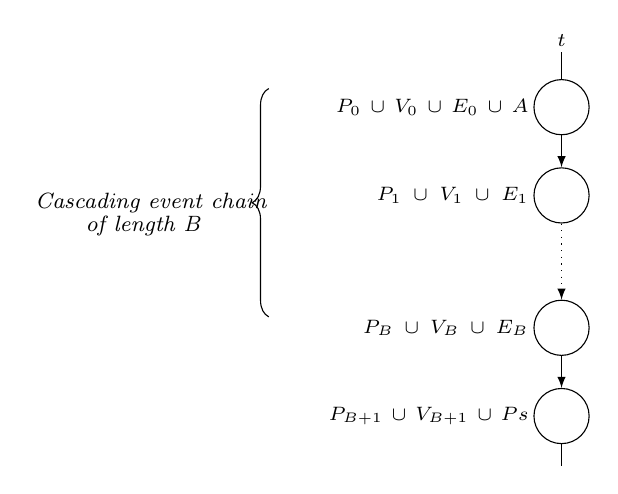
\begin{tikzpicture}[>=latex]
  \begin{scriptsize}
  \begin{scope}

  \node[align=center] (t1) at (0em,3em) {$t$};

  
  \draw (0em,2.5em) -- (0,1.25em);
 

  \node[circle, inner sep=0em, draw, minimum size=2.5em] (b0) at (0em,0) {};
  \node[align=right, text width=12em] (b0e) at (-7.5em,0) {$P_{0}\cup V_{0}\cup E_{0}\cup A$};

  \node[circle, inner sep=0em, draw, minimum size=2.5em] (b1) at (0em,-4em) {};
  \node[align=right, text width=12em] (b1e) at (-7.5em,-4em) {$P_{1}\cup V_{1}\cup E_{1}$};

  \node[circle, inner sep=0em, draw, minimum size=2.5em] (b2) at (0em,-10em) {};
  \node[align=right, text width=12em] (b2e) at (-7.5em,-10em) {$P_{B}\cup V_{B}\cup E_{B}$};
 
 \node[circle, inner sep=0em, draw, minimum size=2.5em] (bb) at (0em,-14em) {};
 
 \node[align=right, text width=12em] (bbe) at (-7.5em,-14em) {$P_{B+1}\cup V_{B+1}\cup Ps$};

  
  \draw (0em,-15.25em) -- (0,-16.25em);


  \draw[->] (b0) -- (b1);
  \draw[->, dotted] (b1) -- (b2);
  \draw[->] (b2) -- (bb);
  
  
\draw [decorate,decoration={brace,amplitude=6pt},xshift=-120pt,yshift=-90pt]
(0.5,0.5) -- (0.5,3.4) node [black,midway,xshift=-1.5cm] 
{\footnotesize $\textit{Cascading event chain}$} node [black,midway,xshift=-1.6cm, yshift=-0.3cm] 
{\footnotesize $\textit{of length B}$};

  \end{scope}
  \end{scriptsize}
\end{tikzpicture}

\caption{A single happening occurs at time $t$, and includes several sets of state variables. These sets describe a causal chain of instantaneous events.}
\label{fig:happening}
\end{figure}

Following from Definition~\ref{def:happening}, happening $x_t$ is encoded by the SMT variables:
$$
x_t:=\Bigg \langle 
\begin{array}{l}
\qquad time_t,\\
\qquad P_{0,t},\ldots,\,P_{B+1,t},\\
\qquad V_{0,t},\ldots,\,V_{B+1,t},\\
\qquad E_{0,t},\ldots,\,E_{B,t},\\
\qquad Ps_t,\,A_t,\,\\
\qquad flow_{V_t},\,dur_{Ps_t}
\end{array}
\Bigg \rangle 
$$

The happenings in our encoding either describe a moment of discrete change -  which corresponds to the discrete transition \textit{Trans} of the hybrid automata - or a point in time between moments of discrete change in which the derivative is equal to zero for some numeric continuous change. The latter case is to ensure that invariant conditions hold, avoiding the case described later in Figure~\ref{fig:Zero_cross}. Between happenings there is only continuous numeric change (\textit{Flow}). The key difference between a hybrid automaton and the SMT encoding is that multiple actions can be performed in a single happening in parallel, meaning that while the hybrid automaton is exponential in the size of the PDDL+ description, our encoding will be linear.

The set $flow_{V_{t}}:=\{flow_{{v_t}} | \forall v_t\in V_t\}$ is a set of numeric expressions that represent the change in value of each numeric variable $v$ from this time point to the next. The variables $dur_{{Ps_t}}:=\{dur_{ps_t} | \forall ps_t\in Ps_t\}$ represents the remaining duration of each process. $dur_{ps}$ and is constrained to be positive if and only if the process is currently executing.

The constraints within a happening are shown in Figure~\ref{eq:state}. 

\begin{figure*}[thb!]
% \begin{minipage}[t]{0.58\linewidth}
\textbf{Proposition and real variable support}
\begin{enumerate}[label=H\arabic*.]
 % Literal support
  \item $\bigwedge_{p \in P} p_{1,t} \rightarrow (p_{0,t} \vee \bigvee_{e \in E | p \in eff^{+}_{e}} e_{0,t} \vee \bigvee_{a_t \in A | p \in eff^{+}_{a}} a_t)$
  \item $\bigwedge_{p \in P} \neg p_{1,t} \rightarrow (\neg p_{0,t} \vee \bigvee_{e \in E | p \in eff^{-}_{e}} e_{0,t} \vee \bigvee_{a \in A | p \in eff^{-}_{a}} a_t)$
  \item $\bigwedge_{i=1}^{B} \bigwedge_{p \in P} p_{i+1,t}      \rightarrow (     p_{i,t} \vee \bigvee_{e \in E | p \in eff^{+}_{e}} e_{i,t})$
  \item $\bigwedge_{i=1}^{B} \bigwedge_{p \in P} \neg p_{i+1,t} \rightarrow (\neg p_{i,t} \vee \bigvee_{e \in E | p \in eff^{-}_{e}} e_{i,t})$
 % Real variable support
  \item $\bigwedge_{v \in V} (\bigwedge_{a \in A | v \in eff^{num}_{a}} \neg a_{t} \wedge \bigwedge_{e \in E | v \in eff^{num}_{e}} \neg e_{0,t}) \rightarrow (v_{i+1,t} = v_{i,t})$
  \item $\bigwedge_{i=1}^{B} \bigwedge_{v \in V} (\bigwedge_{e \in E | v \in eff^{num}_{e}} \neg e_{i,t}) \rightarrow (v_{i+1,t} = v_{i,t})$
\end{enumerate}
\textbf{Event preconditions and effects}
\begin{enumerate}[label=H\arabic*.]\setcounter{enumi}{6}
 % event preconditions
 \item $\bigwedge_{i=0}^{B} \bigwedge_{e \in E} e_{i,t} \leftrightarrow pre_{e} (P_{i,t} \cup V_{i,t})$
 % event effects
 \item $\bigwedge_{i=0}^{B} \bigwedge_{e \in E} e_{i,t} \rightarrow eff_{e} (P_{i+1,t} \cup V_{i+1,t})$
\end{enumerate}
% \end{minipage}
% \begin{minipage}[t]{0.42\linewidth}
\textbf{Action preconditions and effects}
\begin{enumerate}[label=H\arabic*.]\setcounter{enumi}{8}
 % Action preconditions
 \item $\bigwedge_{a \in A} a_t \rightarrow pre_{a}(P_{0,t} \cup V_{0,t})$
  % action effects
 \item $\bigwedge_{a \in A} a_t \rightarrow eff_{a}(P_{1,t} \cup V_{1,t})$
\end{enumerate}
\textbf{Process triggering}
\begin{enumerate}[label=H\arabic*.]\setcounter{enumi}{10}
 % process triggering
 \item $\bigwedge_{ps\in Ps} ps_t \leftrightarrow pre_{ps}(P_{B+1,t} \cup V_{B+1,t})$
 \item $\bigwedge_{ps\in Ps} dur_{ps_t} >= 0$
 \item $\bigwedge_{ps\in Ps} ps_t \leftrightarrow (dur_{ps_t} > 0)$
\end{enumerate}
\textbf{Action mutexes}
\begin{enumerate}[label=H\arabic*.]\setcounter{enumi}{13}
 % Action mutexes
 \item $\bigwedge_{a \in A} \bigwedge_{a' \in A | a \nparallel a'} (\neg a_t \vee \neg a'_t)$
\end{enumerate}
% \end{minipage}
\caption{Encoding of a PDDL+ happening to SMT.}
\label{eq:state}
\end{figure*}

\smallskip

\begin{itemize}

\item Proposition and real variable support

These constraints ensure that the value of propositions (H1-H4) and real variables (H5-H6) remains consistent from $P_{0,t}\cup V_{0,t}$ to $P_{B+1,t}\cup V_{B+1,t}$. Constraints (H1) and (H2) enforce the correct values after considering the add and delete effects of the initial events ($E_{0,t}$) and actions (${A_t}$). Similarly, constraints (H3) and (H4) enforce the propositional add and delete effects throughout the instantaneous chain of events. (H5) enforces the numeric effects of the initial events and actions. (H6) enforces the numeric effects of the remaining events. Note that after the first layer at each happening there are only events, and no actions.

\item Event preconditions and effects

This set of constraints enforces that an event is triggered if and only if its precondition holds (H7) and that if an event is triggered, its effects are present in the next layer of that happening (H8).

\item Action preconditions and effects

Similar to (H6-H7), these constraints ensure for actions $A_t$ that their preconditions must hold in $P_{0,t}\cup V_{0,t}$ (H9) and their effects are enforced in $P_{1,t}\cup V_{1,t}$ (H10).

\item Process triggering

This group of constraints enforce that a process is active if and only if its preconditions are satisfied in set $P_{B+1,t}\cup V_{B+1,t}$ (H11). It also enforces that the real variable $dur_{ps_t}$ for each process is greater than or equal to zero (H12), and strictly greater that zero if and only if the process is active at the end of the causal chain of events (H13). These constraints will be used to ensure that a process cannot finish outside of a happening.

\item Action mutexes

This set of binary constraints enforces that no two mutex actions can be applied simultaneously. For each pair of mutex actions, denoted $a_t \nparallel a'_t$, at least one must be false (H14).

\end{itemize}

\subsection{Encoding of a Plan}\label{sec:enc_problem}

Having defined happenings, a PDDL+ problem $\Pi+$ can be encoded as a bounded number of happenings $X:=\{x_1,\ldots,x_n\}$, such that any proof for the SMT formula represents the trace of a valid plan for $\Pi+$. The \textit{plan} corresponding to that trace is the set of action assignments $A_1\cup \ldots\cup A_n$.\footnote{As processes and events do not appear in a PDDL+ plan.}

Therefore, the existence of a plan for a  {\sl PDDL+ planning problem $\Pi+$ with bound $n$} is proved by building the SMT formula $\Pi+_n$ in the theory of quantifier-free (nonlinear) real arithmetic with $n$ copies of the set of happening variables $X = \{x_1,\ldots,x_n\}$ for $n \geq 1$. A \textit{plan for $\Pi+$} is the assignment to the action variables in any proof of $\Pi+_n$. The encoding is illustrated by Figure~\ref{fig:plan}.

\begin{figure*}[thb]
\center
\begin{tikzpicture}[>=latex]
  \begin{scriptsize}
  \begin{scope}

  % Initial and goal

  \node[align=right, text width=4em] (b0e) at (-6em,0) {\large $I$};
  \draw (-3em,0em) -- (2em,0em);
  \node[circle, inner sep=0em, draw, minimum size=0.5em, fill=black] at (2em,0em) {};
  
  \node[align=left, text width=4em] (b0e) at (50em,-5em) {\large $G$};
  \draw (42em,-5em) -- (47em,-5em);
  \node[circle, inner sep=0em, draw, minimum size=0.5em, fill=black] at (42em,-5em) {}; 
  
  % Happening 1
  
  \node[align=center] at (2em,4em) {\large $x_1$};
 
  
  \draw (2em,1.5em) -- (2em,1em);

  \node[circle, inner sep=0em, draw, minimum size=2.0em] (b01) at (2em,0) {};
  \node[circle, inner sep=0em, draw, minimum size=2.0em] (b11) at (2em,-2em) {};
  \node[circle, inner sep=0em, draw, minimum size=2.0em] (bb1) at (2em,-5em) {};


  \draw (2em,-6em) -- (2em,-8em);
  
  \draw[->, dotted] (b11) -- (bb1);
 
  
  % Happening 2

  \node[align=center] at (12em,4em) {\large $x_2$};
 
  
  \draw (12em,1.5em) -- (12em,1em);


  \node[circle, inner sep=0em, draw, minimum size=2.0em] (b02) at (12em,0) {};
  \node[circle, inner sep=0em, draw, minimum size=2.0em] (b12) at (12em,-2em) {};
  \node[circle, inner sep=0em, draw, minimum size=2.0em] (bb2) at (12em,-5em) {};


  \draw (12em,-6em) -- (12em,-8em);

  
  \draw[->, dotted] (b12) -- (bb2);
  
  
  % Happening 3
  
  \node[align=center] at (22em,4em) {\large $x_3$};
  
 
  \draw (22em,1.5em) -- (22em,1em);


  \node[circle, inner sep=0em, draw, minimum size=2.0em] (b03) at (22em,0) {};
  \node[circle, inner sep=0em, draw, minimum size=2.0em] (b13) at (22em,-2em) {};
  \node[circle, inner sep=0em, draw, minimum size=2.0em] (bb3) at (22em,-5em) {};


  \draw (22em,-6em) -- (22em,-8em);
 
  
  \draw[->, dotted] (b13) -- (bb3);
 

  % Happening 4
  
  \node[align=center] at (42em,4em) {\large $x_n$};
  
  \draw (42em,1.5em) -- (42em,1em);


  \node[circle, inner sep=0em, draw, minimum size=2.0em] (b04) at (42em,0) {};
  \node[circle, inner sep=0em, draw, minimum size=2.0em] (b14) at (42em,-2em) {};
  \node[circle, inner sep=0em, draw, minimum size=2.0em] (bb4) at (42em,-5em) {};
 

  \draw (42em,-6em) -- (42em,-8em);

  
  \draw[->, dotted] (b14) -- (bb4);

  
  
  % Inter-happening edges
  
  \draw (bb1) edge[out=0,in=180,->] (b02);
  \draw (bb2) edge[out=0,in=180,->] (b03);
  \draw[dotted] (26em,-4em) -- (37em,-4em);
  
  \end{scope}
  \end{scriptsize}
\end{tikzpicture}
\caption{A plan is found by building a formula with $n$ copies of the set of variables $x_t$ for $t = 1 \ldots n$. Each Happening models discrete change. Between happenings there is only continuous numeric change. The initial state is modelled in $t_1$, and the goal constraints are added to $t_n$.}
\label{fig:plan}
\end{figure*}

\noindent The constraints for a happening in Figure~\ref{eq:state} are copied for each happening $x_1 \ldots x_n$. Additional constraints in the SMT formula $\Pi+_n$ are shown in Figure~\ref{eq:plan} and explained below.

\begin{figure*}[thb]
\begin{minipage}[t]{0.39\linewidth}
\textbf{Instance description}
\begin{enumerate}[label=P\arabic*.]
  % Known states
  \item $I(P_{0,1}\cup V_{0,1})$
  \item $G(P_{B+1,n}\cup V_{B+1,n})$
  % Timing of happenings
  \item $time_1 = 0$
  \item $\bigwedge_{i=2}^n time_i \geq time_{i-1}+\epsilon$
\end{enumerate}
\textbf{Proposition support}
\begin{enumerate}[label=P\arabic*.]\setcounter{enumi}{4}
  % Literal support
  \item $\bigwedge_{i=2}^n \bigwedge_{p\in P} p_{0,i} \rightarrow p_{B+1,i-1}$
  \item $\bigwedge_{i=2}^n \bigwedge_{p\in P} \neg p_{0,i} \rightarrow \neg p_{B+1,i-1}$
\end{enumerate}
\end{minipage}
\begin{minipage}[t]{0.6\linewidth}
\textbf{Invariants}
\begin{enumerate}[label=P\arabic*.]\setcounter{enumi}{6}
  % Process timing conditions (these are necessary in combination to ensure happenings occur at dur=0)
  \item $\bigwedge_{i=2}^n \bigwedge_{ps\in Ps} ps_{i-1} \rightarrow dur_{ps_i} = dur_{ps_{i-1}} - time_i + time_{i-1}$
  % Interval constraints
  \item $\bigwedge_{i=1}^{n-1} \bigwedge_{ps \in Ps}  ps_i \leftrightarrow pre_{\leftrightarrow ps_i}$
  \item $\bigwedge_{i=1}^{n-1} \bigwedge_{e\in E} \neg pre_{\leftrightarrow e_i}$
\end{enumerate}
\textbf{Continuous change on real variables}
\begin{enumerate}[label=P\arabic*.]\setcounter{enumi}{9}
 % Vector flows
  \item $\bigwedge_{i=1}^{n-1} \bigwedge_{v\in V} flow_{v_i} = \int^{time_{i+1}}_{time_i} \sum_{ps\in Ps} eff^{num}_{\leftrightarrow ps}(V_i)dt$
  \item $\bigwedge_{i=2}^n \bigwedge_{v\in V} (v_{0,i} = v_{B+1,i-1} + flow_{v,i-1})$
\end{enumerate}
\end{minipage}
\caption{Encoding of PDDL+ planning problem $\Pi+$ to SMT.}
\label{eq:plan}
\end{figure*}

% According to the PDDL2.1 and PDDL+ epsilon separation semantics, effects can be exploited by actions $\epsilon$ time after they occur, therefore we need to apply the changes at time point $t+\epsilon$. Formally, we have the following 

\begin{itemize}

\item Instance description

These constraints enforce the initial state to hold in the first happening (P1), and that the goal is achieved in the final happening (P2). Following PDDL2.1 and PDDL+ semantics, they constrain the timing of happenings to enforce epsilon separation (P3-P4).

\item Proposition support

These constraints ensure that the discrete state variables do not change between happenings (P5-P6).

\item Invariants

These constraints ensure that the continuous numeric change between happenings does not violate any invariant constraints. First (P7) ensures that if a process is active in the previous happening, its duration is decreased by the time between happenings. This constraint, in combination with constraints (H12-H13) of Figure~\ref{eq:state}, ensure that a process cannot end between happenings. A process can remain active over intervals spanning multiple happenings.

Constraint (P8) enforces the invariant of the process. If a process is active, then the precondition of the process is active over the whole interval between happenings, and if the process is not active, then its preconditions are false over the whole interval. For constraints over real valued variables, this is done by checking the value either side of the interval. For nonlinear change, this is not sufficient (as shown in Figure~\ref{fig:Zero_cross}). It is necessary to include the following additional constraint:
$$
ps_{t_j} \rightarrow \bigwedge^{A_{t_j}}_{a_{t_j}=1} \left((\frac{d^af}{dt^a})_j(\frac{d^af}{dt^a})_{j+1} >= 0\right); 
$$
where $f$ is the numeric, non-constant part of the invariant, and where the $(A+1)$th derivative of $f$ is identically zero. This ensures that the derivatives of the function do not cross zero over the interval, thus a fluctuating value of $f$ cannot violate the invariant condition between $t_j$ and $t_{j+1}$. This is explained in more detail in Section~\ref{sec:enc_zerocrossing}.

\begin{figure*}[htb!]
\center

\usepgfplotslibrary{fillbetween}

\begin{tikzpicture}[domain=-2:2]

%\draw[->] (-3.5,0) -- (3.5,0)
%node[below right] {$x$};
%\draw[->] (0,-2) -- (0,3.5)
%node[left] {$y$};
%\draw plot[id=x] function{-(x*x)+3};
%\end{tikzpicture}


\begin{axis}[
    xmin=-4, xmax=4,
    ymin=-4, ymax=4
    ]

    \addplot [name path=plot1, ultra thin, domain=-10:10, samples=150]{-(x*x)+2}; 
    \addplot [name path=plot2, ultra thin, domain=-8:8]{1};
\addplot[thick, samples=50, smooth,domain=-4:4,magenta, name path=three] coordinates {(2,-4)(2,4)} ;
\addplot[thick, samples=50, smooth,domain=-4:4,magenta, name path=three] coordinates {(-2,-4)(-2,4)};

    

    \addplot[red] fill between[of=plot1 and plot2, soft clip={domain=-1:1}];
    

\end{axis}
\end{tikzpicture}
\caption{The plot illustrates continuous non-linear numeric change between two time points, indicated by vertical lines. While considering the non-linear change, we need to check whether the invariant condition of a process is satisfied throughout the interval. If the invariant asserts that the function should remain below the horizontal line, the figure shows that it is not sufficient to check the value of the function only at the time points.}
\label{fig:Zero_cross}
\end{figure*}

Constraint (P9) similarly ensures that an event is not triggered during an interval.

\item Continuous change on real variables

These constraints enforce continuous change over the interval (P10), applying the result to each real variable (P11). In order to calculate the change, the indefinite integral of the process' effects upon the variable must be computed. This is done automatically using the computer algebra systems (CAS) SymPy~\cite{sympy} and Piranha~\cite{bis18}.

For example, consider the process of the ball falling in the working example. The ball is accelerating at a constant rate in a single axis. The PDDL process describing the continuous change of the ball's velocity and height is as shown in Figure~\ref{fig:ballproc}.

% another example (Free fall)
\begin{figure}[htb!]
\small
\centering
\begin{BVerbatim}
(:process moving
 :parameters (?b - ball)
 :precondition (and (not (holding ?b)) (>= (height ?b) 0))
 :effect (and
    (increase (velocity ?b) (* #t -9.8) )
    (increase (height ?b) (* #t (velocity ?b))))
 )
\end{BVerbatim}
\caption{Simplified PDDL+ Free Fall problem file}
\label{fig:ballproc}
\end{figure}

While this process is active, the change in height of the ball during the interval between two happenings is a non-linear function of time. To enable the encoding to describe this change the CAS first produces an expression for the change in height whose terms are time, and constant coefficients. For example:
$$
\delta h = \frac{1}{2} {at^{2}} + {v_0}t
$$
Where $v_0$ is the initial velocity, and $a$ is the constant acceleration. This is explained in more detail in Section~\ref{sec:example_encodings}, where the whole encoding of the working example is shown.

Note that in this approach, the integration and differentiation required for P8, P9, and P10 are performed outside the solver, during the encoding. Hence the integration is done only once for each domain.
\end{itemize}

\subsection{Continuous Change and the Zero-Crossing Problem}\label{sec:enc_zerocrossing}



\subsection{SMTPlan Architecture} \label{sssec:SMTPlan_Archi}

The encoding has been implemented in a planner, called SMTPlan. The planner follows the procedure of SATPlan, iteratively deepening on the number of happenings (as opposed to the number of steps). The number of happenings can be incremented by step size $s$, which is an integer parameter that the user can specify. Given a planning problem $\Pi$, the algorithm of SMTPlan is as follows:

\begin{enumerate}
\item
Perform the indefinite integration and differentiation on the domain of $\Pi+$.
\item
Encode $\Pi+$ with an initial bound of $n$ happenings, as $\Pi+_n$.
\item
Pass $\Pi+_n$ to SMT solver to attempt to find a satisfying assignment.
\item
If $\Pi+_n$ is unsatisfiable, then $n$ is incremented ($n=n+s$) and the problem is encoded and passed to the solver again.
\item
If satisfiable, then extract the truth assignment to the action variables $A_0, \ldots,\, A_n$ and return.
\end{enumerate}
The algorithm is shown in Algorithm~\ref{alg:pseudo} and the steps described in more detail below. The process is illustrated in figure~\ref{fig:SMTPlan}.

\begin{algorithm}
\SetAlgoLined
\textbf{Input:} Planning Problem $\Pi$, initial bound $n$, step size $s$.\\
$\xi \leftarrow extractExpressions(\Pi)$\tcp*{\small{Extract expressions from domain of $\Pi$.}}
 \Loop{}{
$\Pi_n \leftarrow encode(\Pi,\xi,n)$\tcp*{\small{Extend encoding to $n$ happenings.}}
$M \leftarrow solve(\Pi_n)$\tcp*{\small{Find satisfying assignment.}}
\uIf{$M = \bot$}{
  $n = n + s$\tcp*{\small{Increment the happening bound.}}
}
\Else{
$\pi \leftarrow extractPlan(M)$\tcp*{\small{Extract a plan from the satisfying assignment.}}
\textbf{return};
}
}
\caption{SMTPlan}
\label{alg:pseudo}
\end{algorithm}

\begin{figure}[ht]
\centering
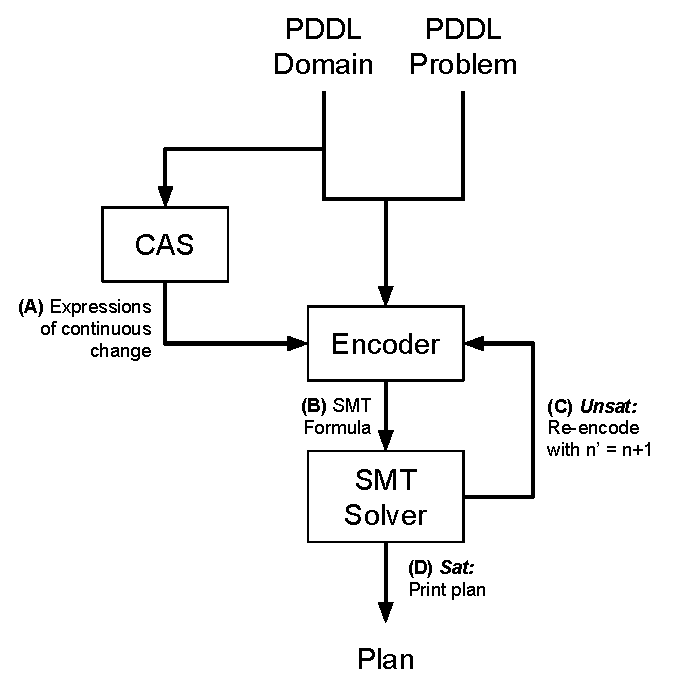
\includegraphics[width=0.50\textwidth]{diagrams/architecture.pdf}
\caption{An overview of the SMTPlan architecture. (A) First the Computer Algebra System performs the indefinite integration and differentiation to produce the expressions of continuous numeric change. (B) The PDDL problem instance is encoded as a SMT formula, with an initial number of happenings $n=2$. The encoding is passed to an SMT solver. (C) If the encoding is unsatisfiable, then the number of happenings is incremented. (D) Finally, if the encoding is satisfiable, the plan is printed. }
\label{fig:SMTPlan}
\end{figure}

The indefinite integration and differentiation required for constraints enforcing the checking of invariant conditions (P8-P9) and continuous numeric change (P10-P11) is performed by extracting the expressions from the PDDL+ domain of $\Pi+$ and passing to the CAS (line 2). In the current implementation of SMTPlan the CAS piranha is used, as it is able to solve polynomial non-linear integrals. The resulting expressions are used in all subsequent encoding steps.

The implementation of the encoding step (line 4) uses the \textit{c++} interface of the SMT-solver z3. This interface allows the planner to incrementally add constraints and call the solver. The benefit of this incremental solving is that each happening only needs to be encoded once, and the iterations are encoded in time linear to the size of the happening and independent of the number of happenings. For example, if an encoding with $4$ happenings was found to be unsatisfiable, then extending the encoding to $5$ happenings only requires adding the variables and constraints of happening $x_5$ to the $z3$ interface.

Extracting the plan from the satisfying assignment (line 9) is performed by simply printing all the variables $a\in A_i$ for each $i=1\ldots n$ that are assigned \textit{true}. This corresponds with the actions applied in each happening in order to achieve the goal.

